\documentclass{jsarticle}
\usepackage[dvipdfmx]{graphicx}
\usepackage{float,url}
\usepackage{amsmath} % assumes amsmath package installed
\usepackage{amssymb}  % assumes amsmath package installed
\usepackage{amsfonts}  % assumes amsmath package installed
\usepackage{amsthm}  % assumes amsmath package installed

\title{研究提案書}

\author{物理統計学分野B4 松山拓生 \\ matsuyama.hiroki.24c@st.kyoto-u.ac.jp}
\date{\today}
\begin{document}

\maketitle

\begin{abstract}
Benyond5Gで要求される仕様の一つとして超多数同時接続(mMTC)が挙げられる。この要件を満たしうる通信方式としてカオスベースのICA通信があるが、シュミレーション上での評価にとどまっている。今回は実機を用いてこの方式の検証、評価を行う。
\end{abstract} 

\section{背景}
無線通信技術、現在5Gが徐々に生活に浸透してきているということもあり、非常にホットな分野である。現状5Gで使用されている無線通信技術の元となっているのはCDMA\cite{cdma-overview}であるが、これは3Gの時代から使用されている技術であり、非常に歴史が長い。しかしながら次なるBeyond5G/6Gでは超多数同時接続\cite{mmtc}(mMTC = massive Machine-Type Communications)が求められており、さらなる同時接続可能数の増加を可能とするような無線通信技術が必要となる。

今回紹介するICA通信\cite{red-book}はこのCDMAと同じレイヤーに属する通信方式であり、ブラインド信号源分離と呼ばれる分野の一つである。この通信方式を実際に実機で検証し、各種通信性能の検証を行う。この詳細については次章で説明する。

\section{方法}
\subsection{モデル化}
元信号$\textbf{s}(t) = [s_1(t) \cdots s_n(t)]^t$、混合行列$A\in \mathbb{R}^{n\times n}$、混合信号$\textbf{x}(t) = [x_1(t) \cdots x_n(t)]^t$を用いて
\begin{gather}
    \textbf{x}(t) = A\textbf{s}(t)
\end{gather}
とする。このとき、ある復元行列$B\in \mathbb{R}^{n\times n}$を用いて復元信号$\textbf{y}(t)= [y_1(t) \cdots y_n(t)]^t$を
\begin{gather}
    \textbf{y}(t) = B\textbf{x}(t)
\end{gather}
のように書くことができるが、$\textbf{y}(t)$が現信号$\textbf{s}(t)$に似た特徴をもったベクトルとなるような$B$を見つけられれば、信号がうまく分離できたと考えることができよう。ブラインド信号源分離問題はこのように行列$B$を推定する問題としてモデル化することができる。

\subsection{ICA通信}
ICA通信ではこの問題を信号間の独立性を仮定することによって解くことを考える。現状で利用を考えているのはFastICA\cite{fastica}とEASI\cite{easi}であり、これらはすでに実装し、シュミレーションで分離性能を確認している。(詳細については\ref{sec:now}章で説明する)

\subsection{使用する実機}
analog devicesの提供するadalm-pluto
(\url{https://wiki.analog.com/university/tools/pluto})
を使用して無線通信を行う。これはソフトウェア無線キット(以下SDRと呼ぶ)と呼ばれるものの一種で、ソフトウェアのみで様々な通信方式を実現できる。身近なところではFMラジオを受信したり、ワンセグを受信することも可能である。今回はこのSDRを使用してカオスベースのICA通信という新しい通信方式に対し、実機での検証を行う。

利用方法としては以下のように受信器、送信機をそれぞれ2つずつ使用して検証を行うことを考えている。(モデルにおいて$n=2$)

\begin{figure}[!htbp]
    \begin{center}
        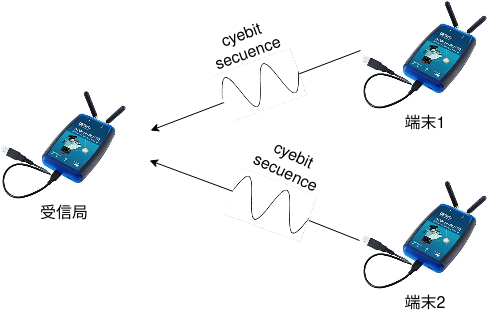
\includegraphics[width=10cm]{img/3device.png}
        \caption{実験概要}
        \label{img:3device}
    \end{center}
\end{figure}

受信端末は基地局、送信端末は各端末としての役割を持つ。これらの送信端末が送信するデータがの受信側で分離の可否を確認するのが、今回の研究の最終目的となる。

\subsection{評価}
通信性能の評価に用いられる指標としてBER(符号誤り率)がある。これは受信した誤り符号の数を送信された符号の総数で割ったものである。今回はこれを使用して各ICAアルゴリズムや送信データに対し、評価を行う。

\section{現状}
\label{sec:now}
現状得ている結果についてもまとめておく。現状では様々なタイプの混合信号に対し、2つのICAアルゴリズム(FastICA\cite{fastica}とEASI\cite{easi})を利用して分離がうまく行くかどうかをコンピューター上で検証している。その結果の一部を以下に記す。

\begin{figure}[H]
    \begin{center}
        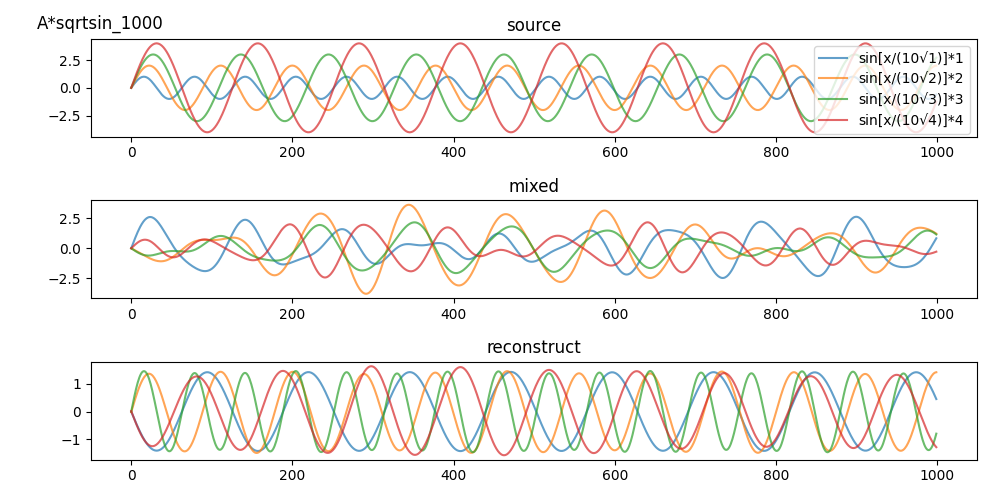
\includegraphics[width=13cm]{img/sqrtsin-fastica.png}
        \caption{正弦波+FastICA(時系列データ)}
        \label{img:sqrtsin-fastica}
    \end{center}
\end{figure}
\begin{figure}[H]
    \begin{center}
        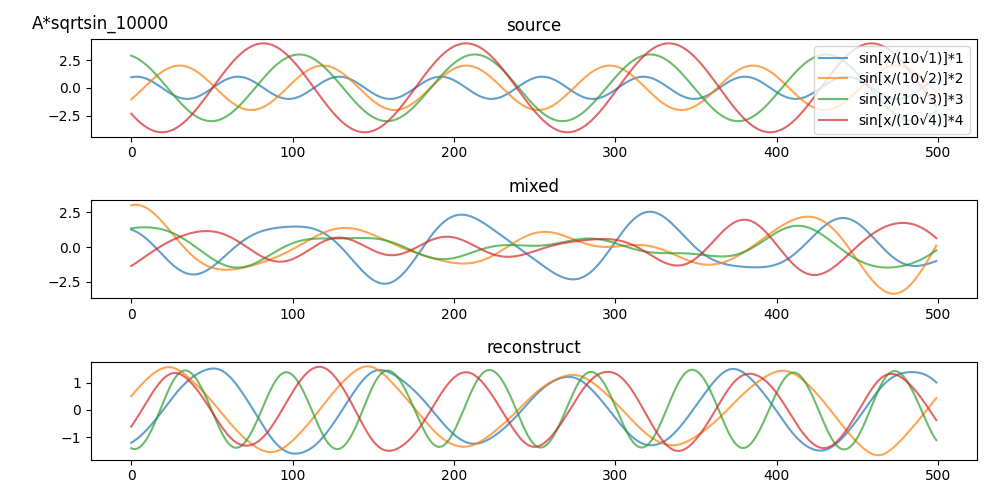
\includegraphics[width=13cm]{img/sqrtsin-easi.png}
        \caption{正弦波+EASI(時系列データ)}
        \label{img:sqrtsin-easi}
    \end{center}
\end{figure}
\begin{figure}[H]
    \begin{center}
        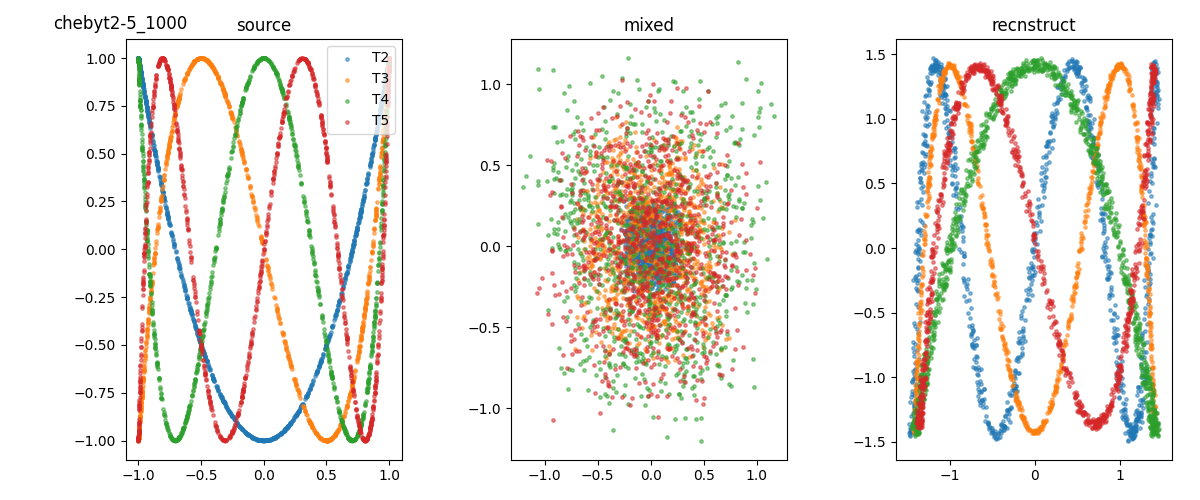
\includegraphics[width=13cm]{img/cyebit-fastica.png}
        \caption{チェビシェフ系列+FastICA(リターンマップ)}
        \label{img:cyebit-fastica}
    \end{center}
\end{figure}
\begin{figure}[H]
    \begin{center}
        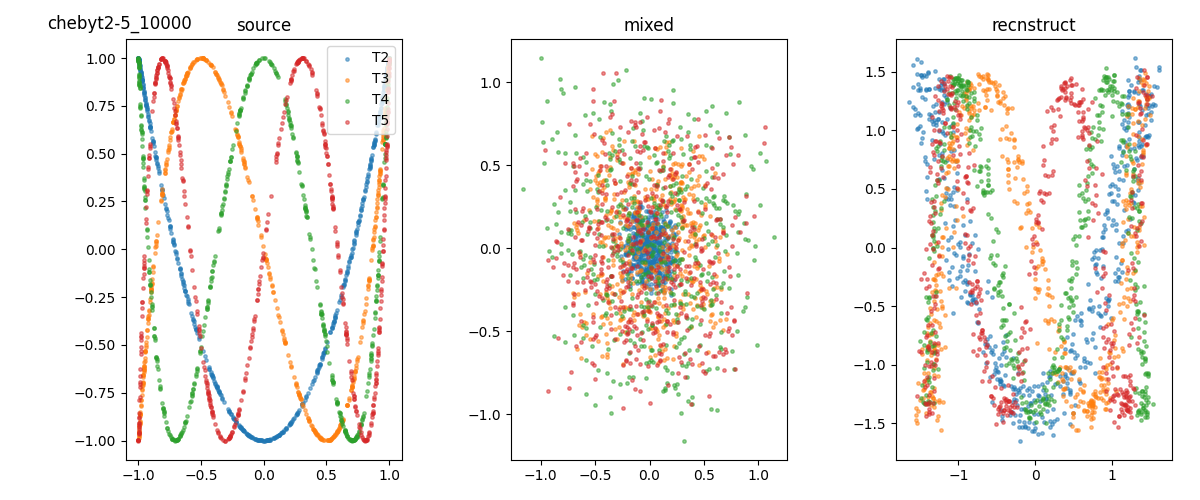
\includegraphics[width=13cm]{img/cyebit-easi.png}
        \caption{チェビシェフ系列+EASI(リターンマップ)}
        \label{img:cyebit-easi}
    \end{center}
\end{figure}
\begin{figure}[H]
    \begin{center}
        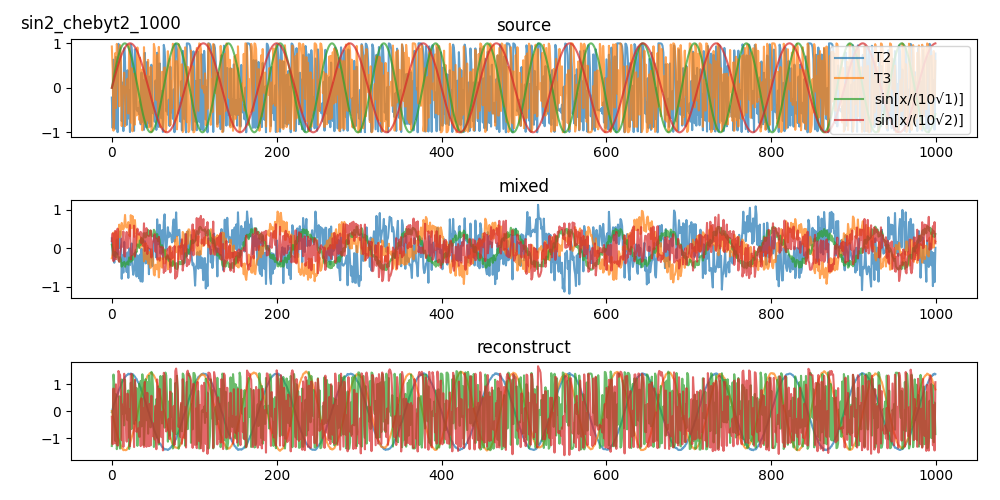
\includegraphics[width=13cm]{img/sinchebyt-plot-fastica.png}
        \caption{チェビシェフ系列&正弦波+FastICA(時系列データ)}
        \label{img:sinchebyt-plot-fastica}
    \end{center}
\end{figure}
\begin{figure}[H]
    \begin{center}
        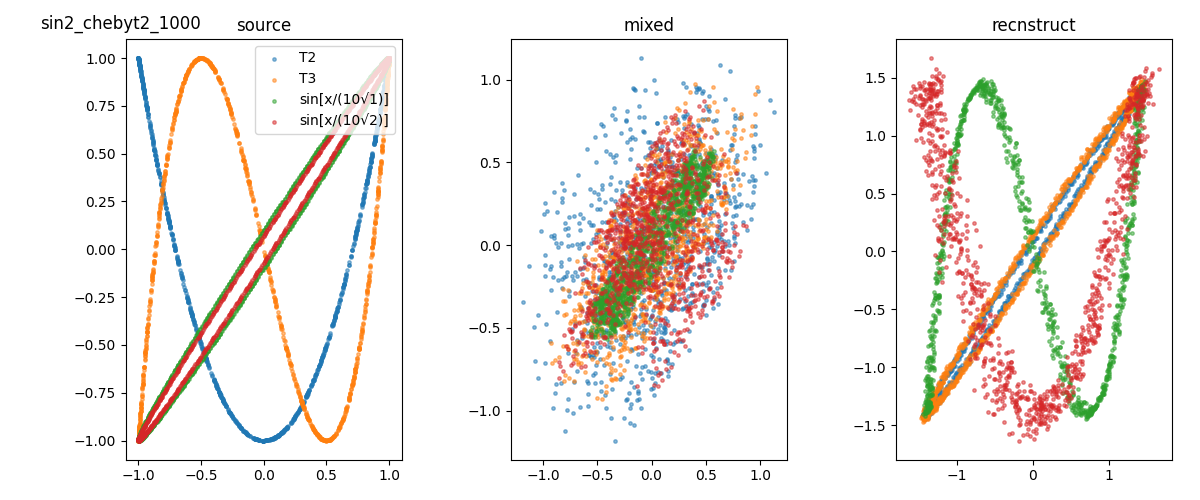
\includegraphics[width=13cm]{img/sinchebyt-ret-fastica.png}
        \caption{チェビシェフ系列&正弦波+FastICA(リターンマップ)}
        \label{img:sinchebyt-ret-fastica}
    \end{center}
\end{figure}

図\ref{img:sqrtsin-fastica}-\ref{img:sinchebyt-ret-fastica}の時系列データにおける横軸は、サンプル数を表す。またFastICAでは1000点をサンプリングしたそのすべてを、EASIでは10000点をサンプリングし、最後の500点のみをそれぞれプロットしている。また、混合行列$A$は$-0.5$から$0.5$における乱数によって生成された行列を用いている。

上記グラフから、FastICA、EASIともに非常に高いパフォーマンスで信号分離が行えていることが分かる。中でも正弦波、チェビシェフ系列の混合がうまく分離できていることは注目に値し、異なる通信方式が共存できる可能性をも示唆している。

\section{展望}

mMTC\cite{mmtc}が課題として挙げられるBeyond5G/6Gでは、IoTなどによる同時接続端末数の劇的な増加に耐えられるような手法が求められる。そのため、2端末での分離が確認できればさらに多くの端末での分離が可能であるかを確認するべきであろう。また、通信の質、通信用モジュールの製造コストを考えると、これらに直結するであろうICAアルゴリズムの見直しも必要であると考えている。オンラインアルゴリズムなどによりメモリの消費を抑え、かつ簡単な演算のみで実装が可能である上に分離性能のよいアルゴリズムについて、まだ研究、調査の余地があるであろう。今後はこのような点から研究を行っていきたいと考えている。

\begin{thebibliography}{99}
    \bibitem{cdma-overview} S. Hara and R. Prasad, Overview of multicarrier CDMA, IEEE Communications Magazine, 126-133, Dec. 1997
    \bibitem{red-book} 梅野 健, 複雑系と通信, 複雑系としての情報システム,
    共立出版, 2007, 181
    \bibitem{mmtc} ANUTUSHA DOGRA and RAKESH KUMAR JHA and SHUBHA JAIN, A Survey on Beyond 5G Network With the Advent of 6G: Architecture and Emerging Technologies
    \bibitem{fastica} A. Hyvarinen, Fast and robust fixed-point algorithms for independent component analysis, IEEE Transactions on Neural Networks ( Volume: 10, Issue: 3, May 1999), 626-634
    \bibitem{easi} J.-F. Cardoso and B.H. Laheld, Equivariant adaptive source separation, IEEE Transactions on Signal Processing ( Volume: 44, Issue: 12, Dec 1996), 3017-3030
\end{thebibliography}

\end{document}